%%%%%%%%%%%%%%%%%%%%%%%%%%%%%%%%%%%%%%%%%%%%%%%%%%%%%%%%%%%%%%%%%%%%%%%%%%%%%%%%
%2345678901234567890123456789012345678901234567890123456789012345678901234567890
%        1         2         3         4         5         6         7         8

\documentclass[letterpaper, 10 pt, conference]{ieeeconf}  % Comment this line out if you need a4paper

%\documentclass[a4paper, 10pt, conference]{ieeeconf}      % Use this line for a4 paper

\IEEEoverridecommandlockouts                              % This command is only needed if 
                                                          % you want to use the \thanks command

\overrideIEEEmargins                                      % Needed to meet printer requirements.

%In case you encounter the following error:
%Error 1010 The PDF file may be corrupt (unable to open PDF file) OR
%Error 1000 An error occurred while parsing a contents stream. Unable to analyze the PDF file.
%This is a known problem with pdfLaTeX conversion filter. The file cannot be opened with acrobat reader
%Please use one of the alternatives below to circumvent this error by uncommenting one or the other
%\pdfobjcompresslevel=0
%\pdfminorversion=4

% See the \addtolength command later in the file to balance the column lengths
% on the last page of the document

% The following packages can be found on http:\\www.ctan.org
\usepackage{graphicx} % for pdf, bitmapped graphics files
\usepackage{subcaption}
\usepackage{blindtext}
%\usepackage{epsfig} % for postscript graphics files
%\usepackage{mathptmx} % assumes new font selection scheme installed
%\usepackage{times} % assumes new font selection scheme installed
%\usepackage{amsmath} % assumes amsmath package installed
%\usepackage{amssymb}  % assumes amsmath package installed

\title{\LARGE \bf
Data Driven Inverse Kinematics using Local Models
}


\author{Fredrik Holsten$^{1}$, Sune Darkner$^{1}$, Morten Pol Engell-Nørregård$^{2}$ and Kenny Erleben$^{1}$% <-this % stops a space
\thanks{$^{1}$Department of Computer Science, University of Copenhagen, Denmark}%
\thanks{$^{2}$Evil Hippie Design}%
}


\begin{document}



\maketitle
\thispagestyle{empty}
\pagestyle{empty}


\begin{abstract}

\blindtext[2]

\end{abstract}



\section{Introduction}
\blindtext[5]
\clearpage

\section{LearningCube}
\blindtext[1]
\begin{figure}[htpb]
      \centering
      \framebox{\parbox{3in}{
        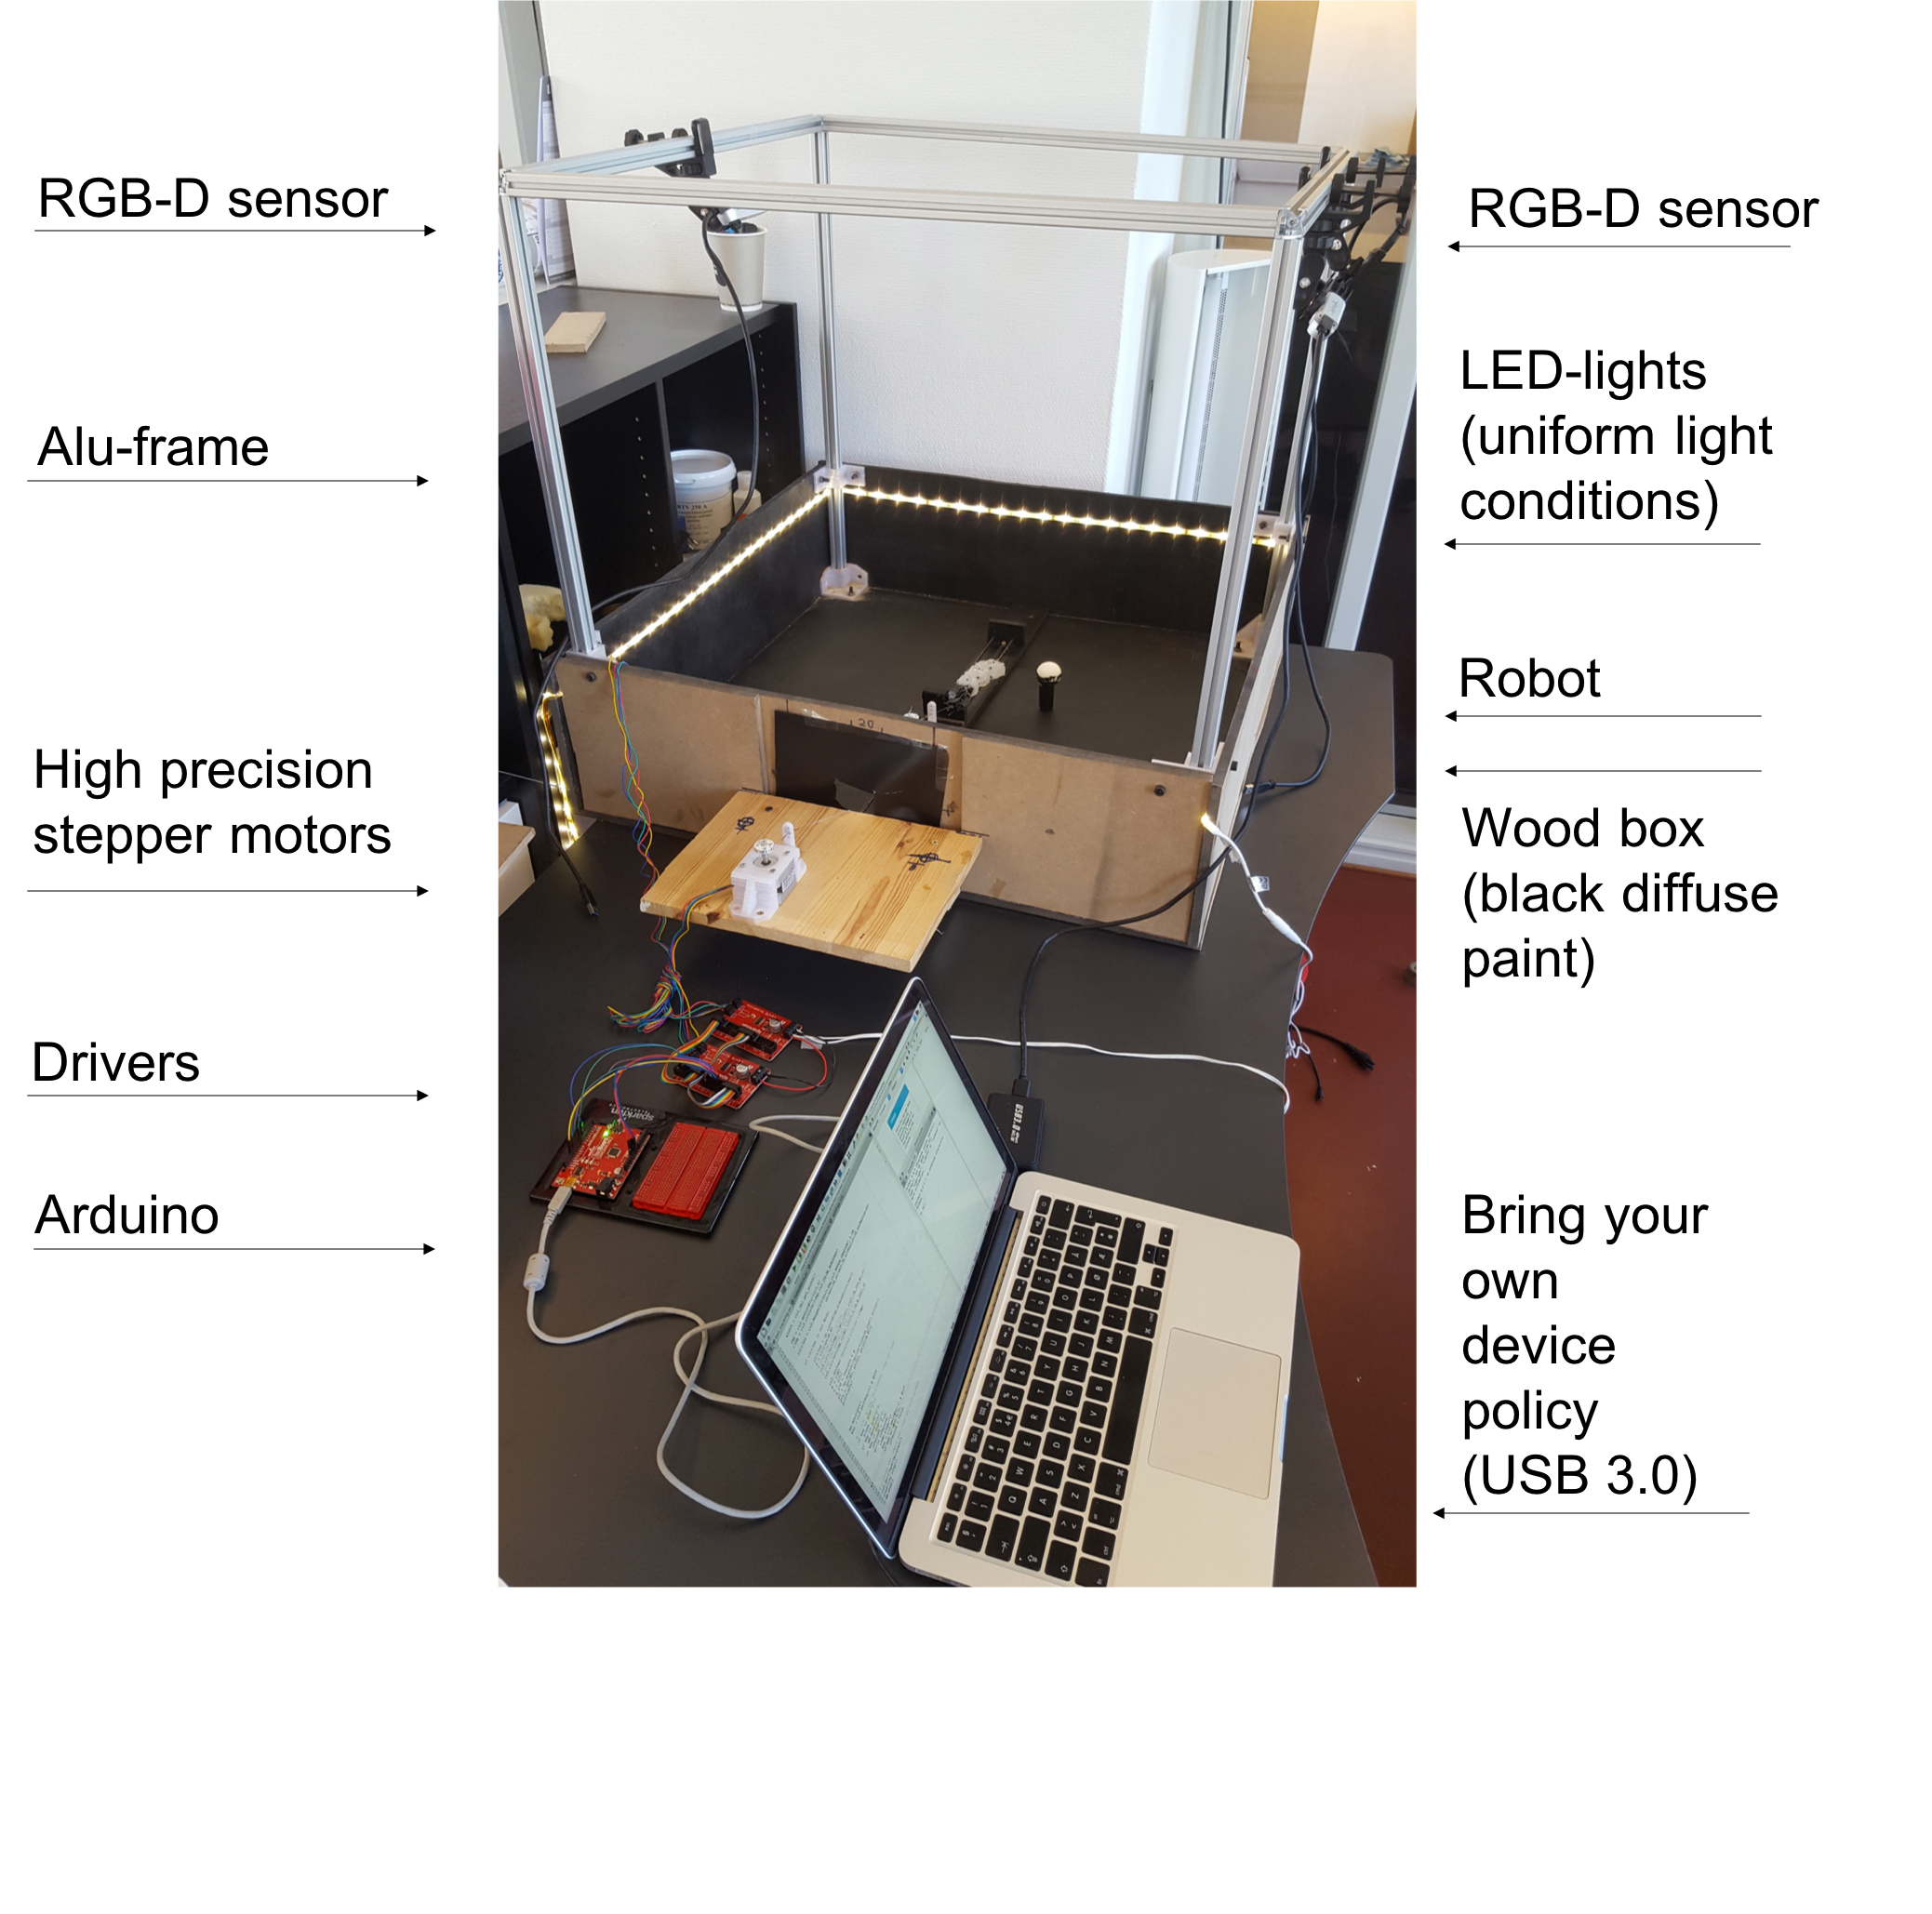
\includegraphics[width=3in,trim={0 5cm 0 0},clip]{figures/learningCube.png}}}
        \caption{Overview of the LearningCube}
        \label{fig:cube}
\end{figure}

\begin{figure}[htpb]
      \centering
      \framebox{\parbox{3in}{
        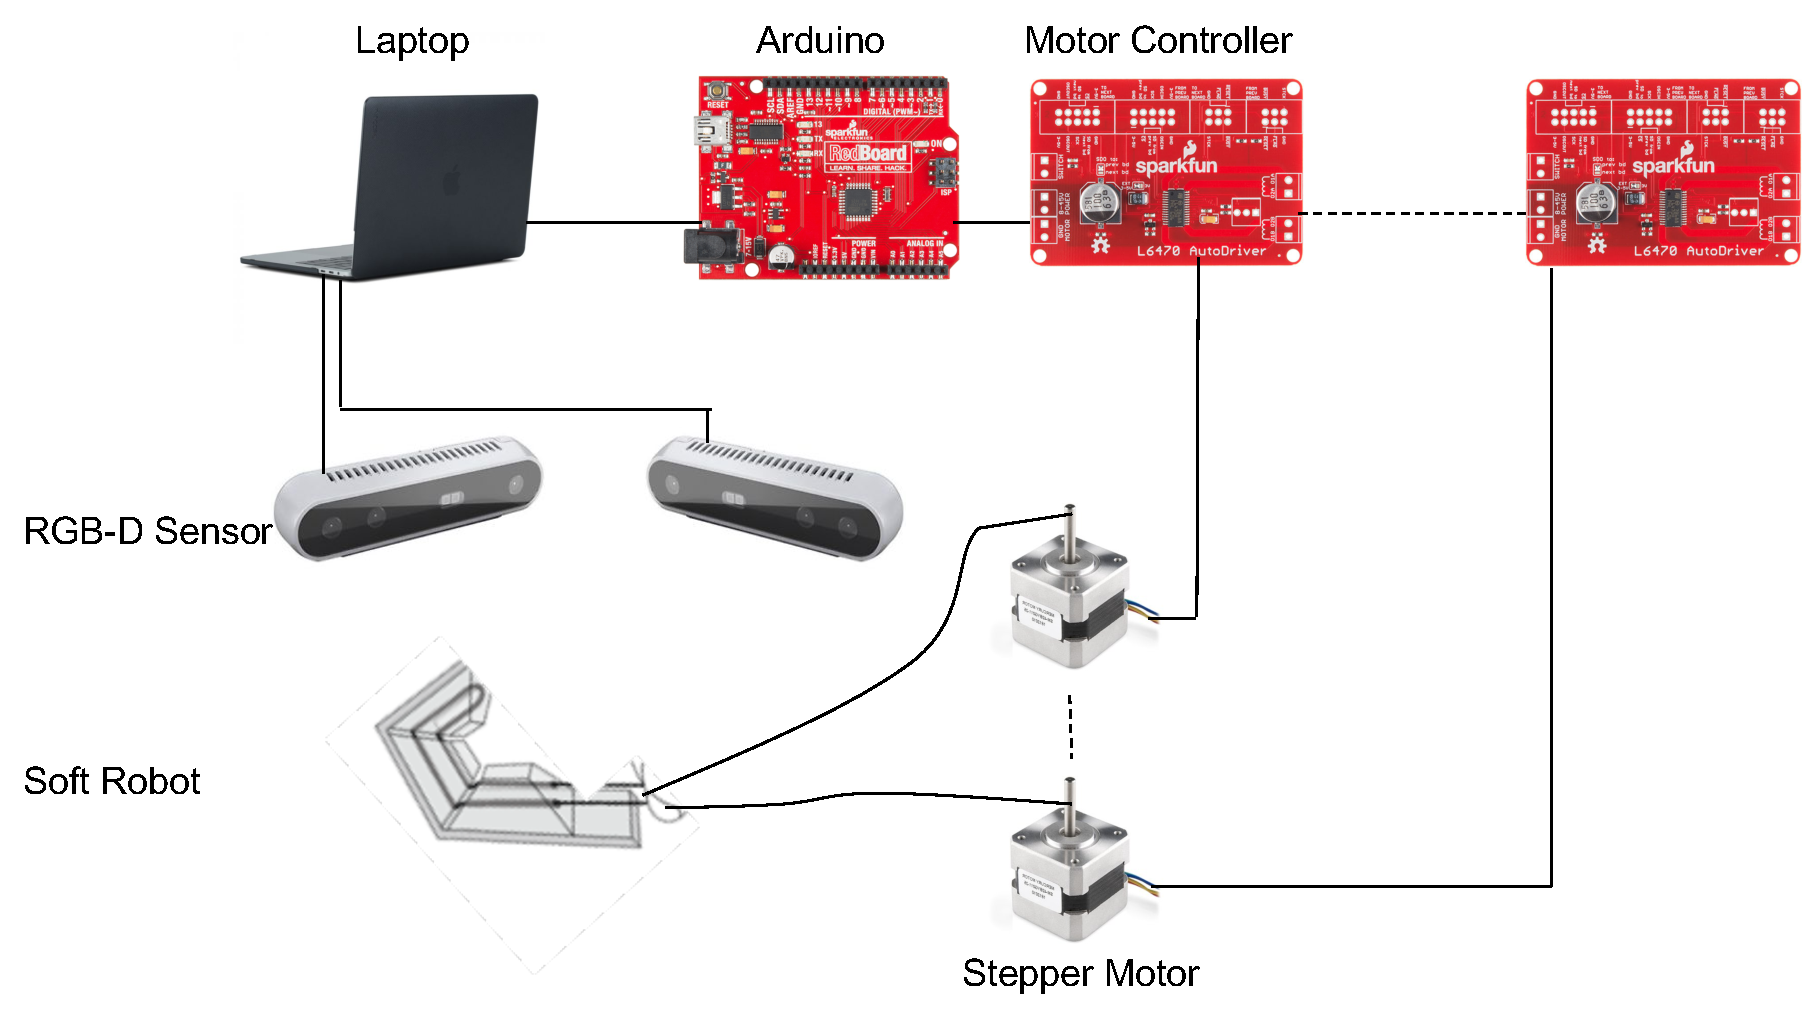
\includegraphics[width=3in]{figures/setup.pdf}}}
        \caption{Overview of the LearningCube}
        \label{fig:cube}
\end{figure}
\blindtext[2]
\begin{figure}[htpb]
      \centering
      \framebox{\parbox{3in}{
        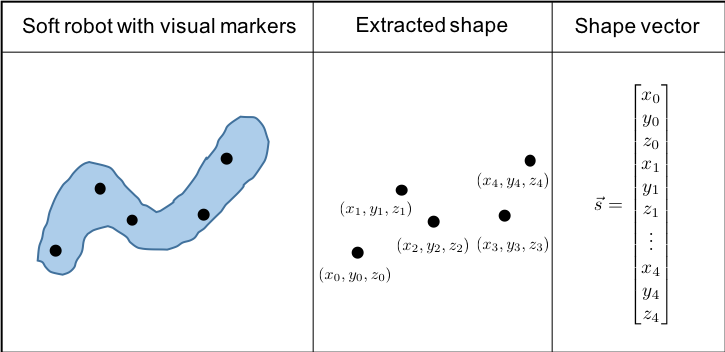
\includegraphics[width=3in]{figures/postiver.png}}}
        \caption{Overview of the LearningCube}
        \label{fig:cube}
\end{figure}

 \begin{figure}[htpb]
        \centering
        \framebox{\parbox{3in}{
        \begin{subfigure}[b]{1.4in} 
                \centering
                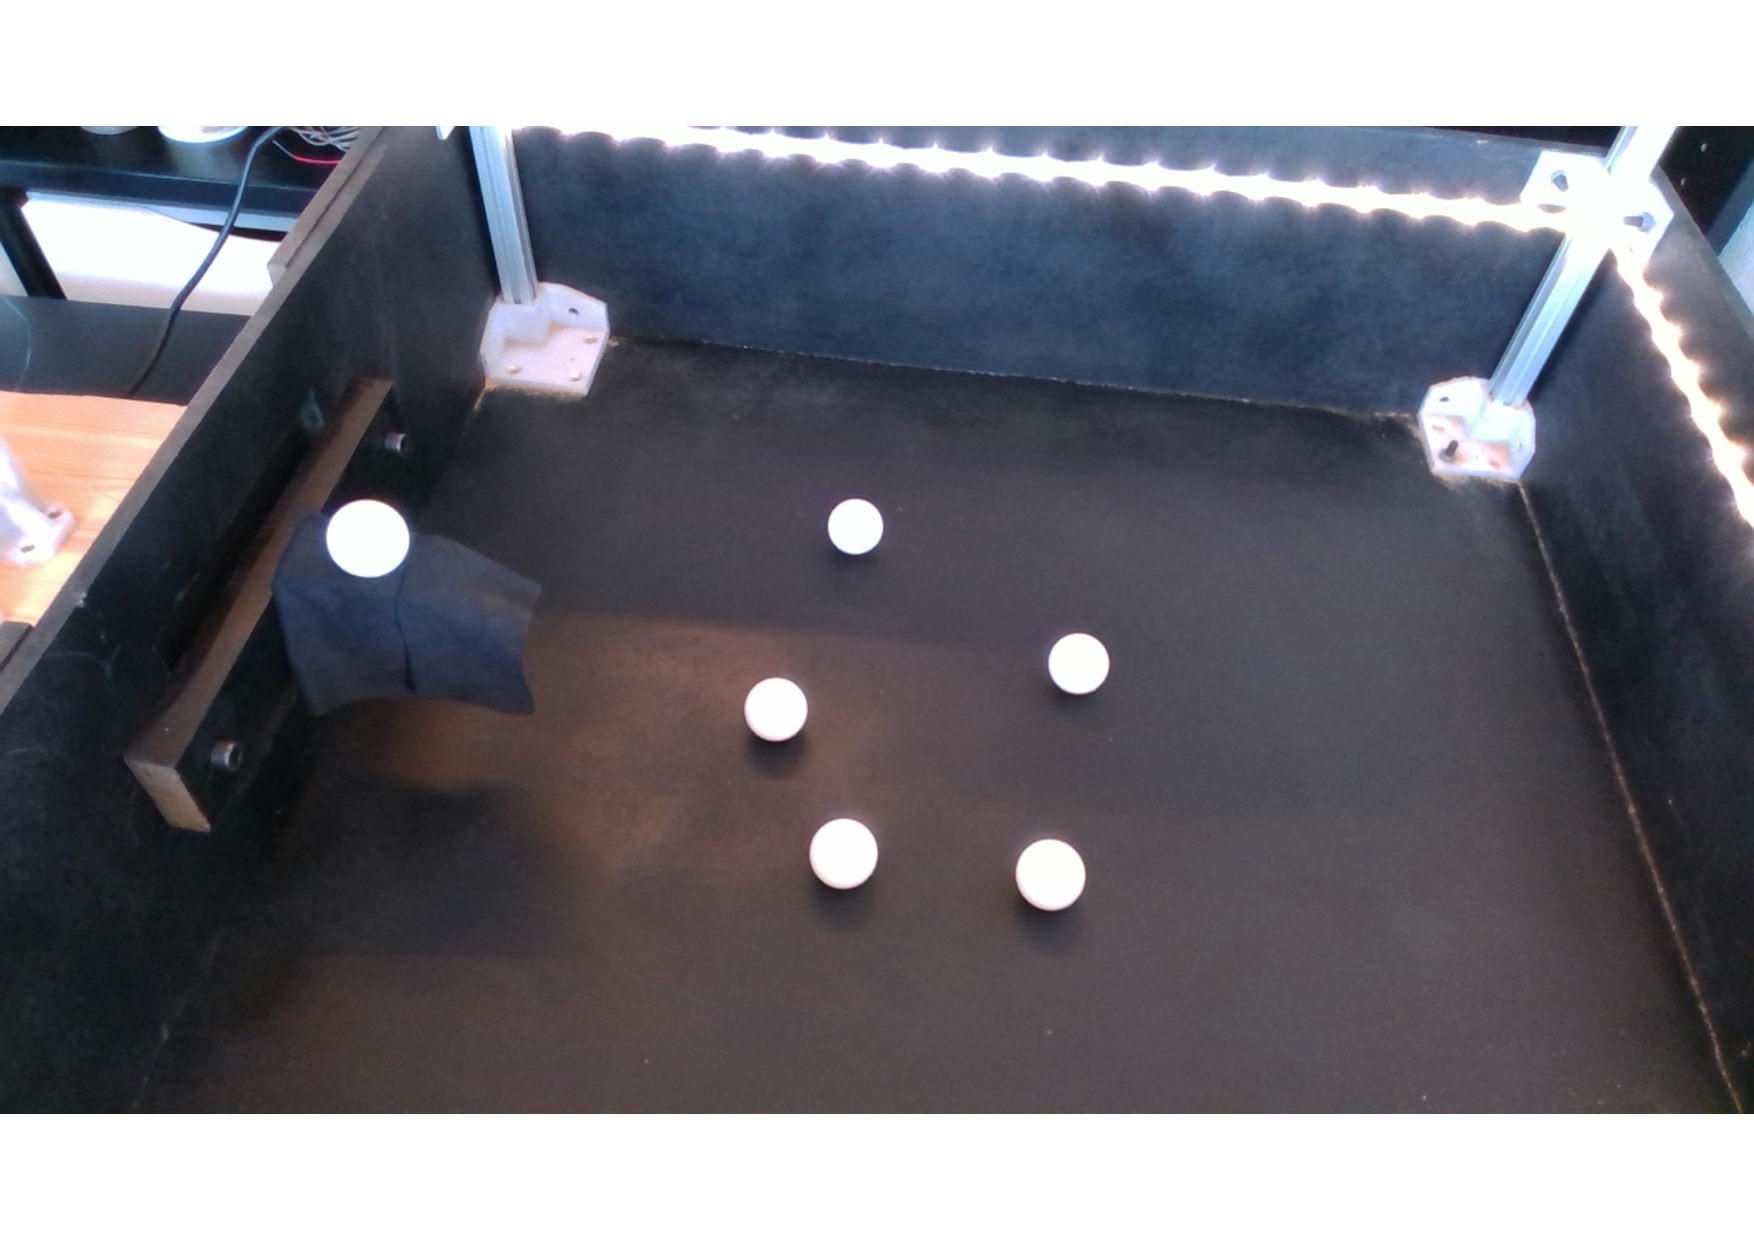
\includegraphics[width=\textwidth]{figures/calib1.pdf}
        \end{subfigure}
        \begin{subfigure}[b]{1.4in}                            
                \centering
                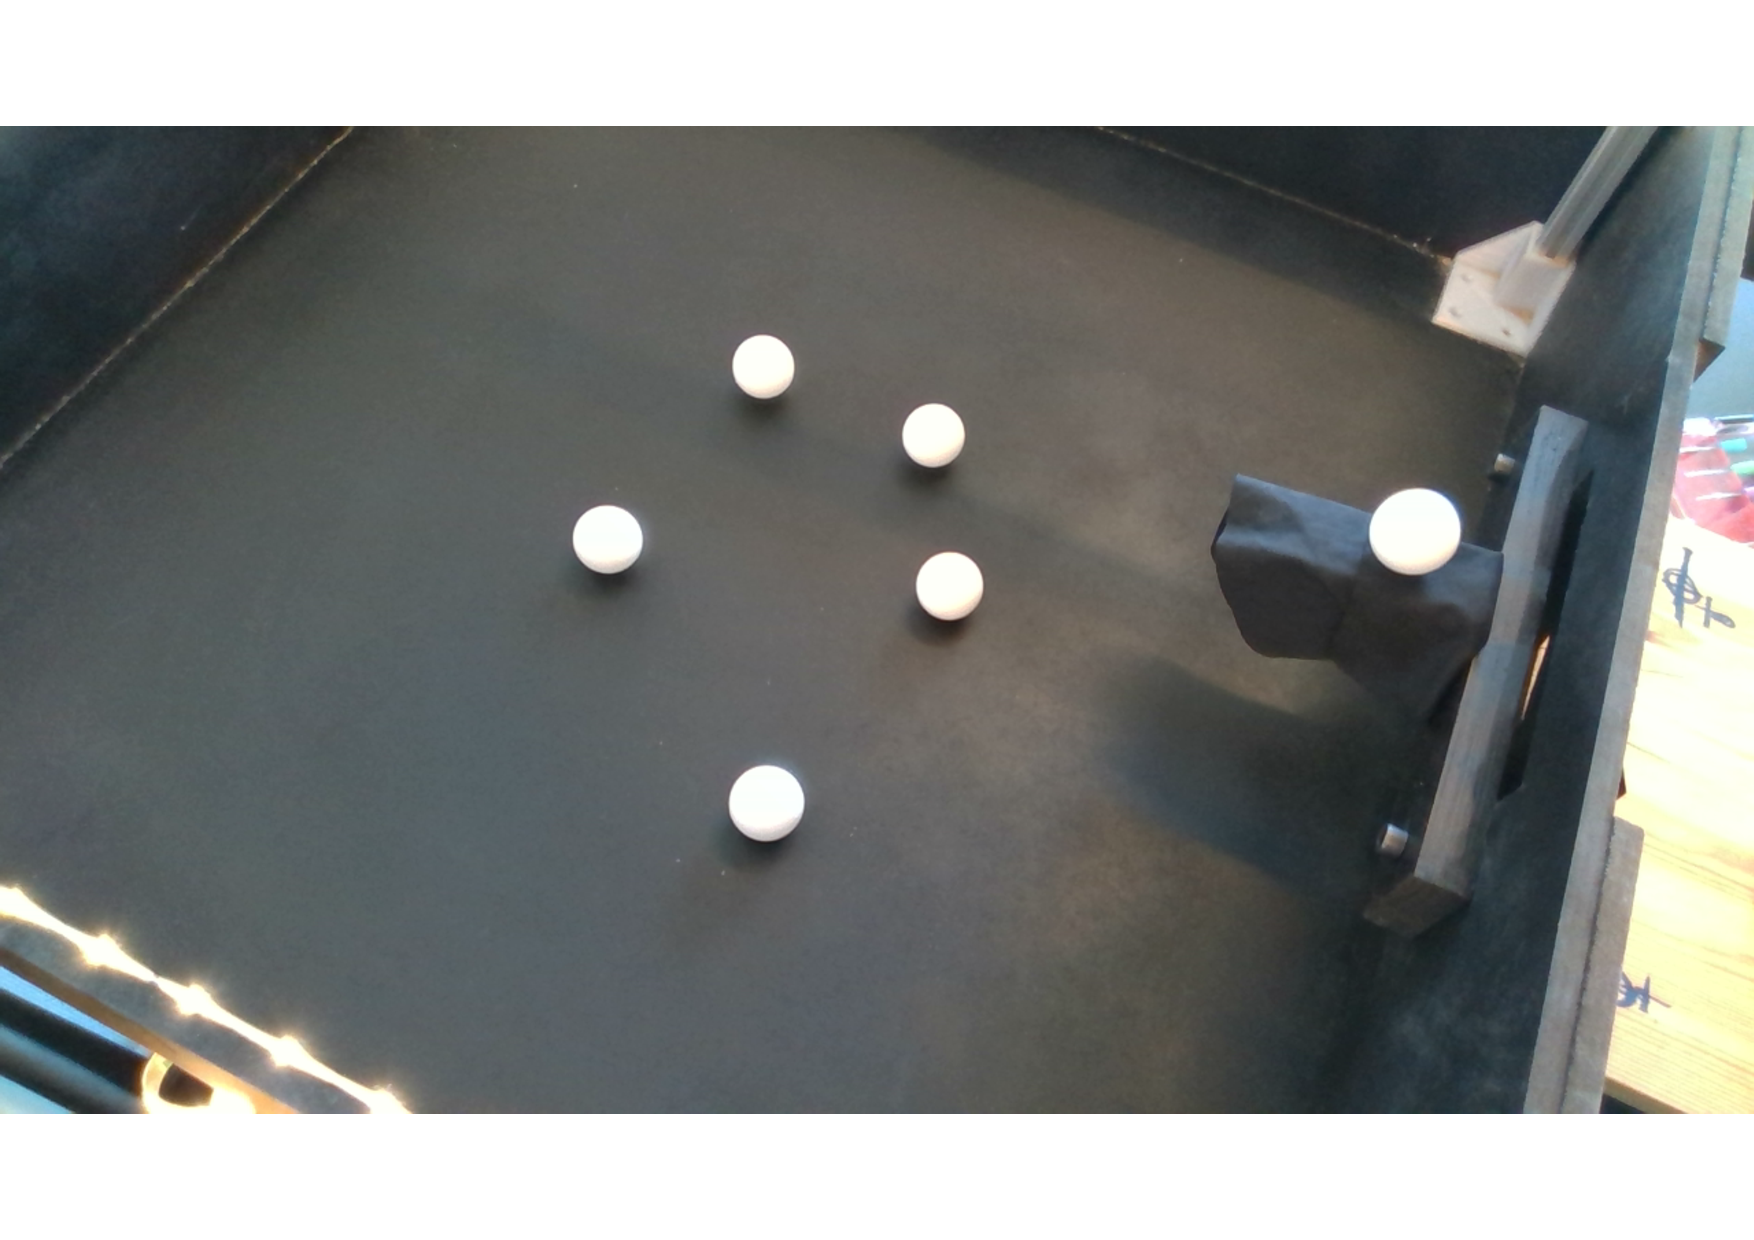
\includegraphics[width=\textwidth]{figures/calib2.pdf}
        \end{subfigure}}}
        \caption{Calibration balls seen from two sensors}
        \label{fig:calib}
\end{figure}

 \begin{figure}[htpb]
        \centering
        \framebox{\parbox{3in}{
        \begin{subfigure}[b]{1.4in} 
                \centering
                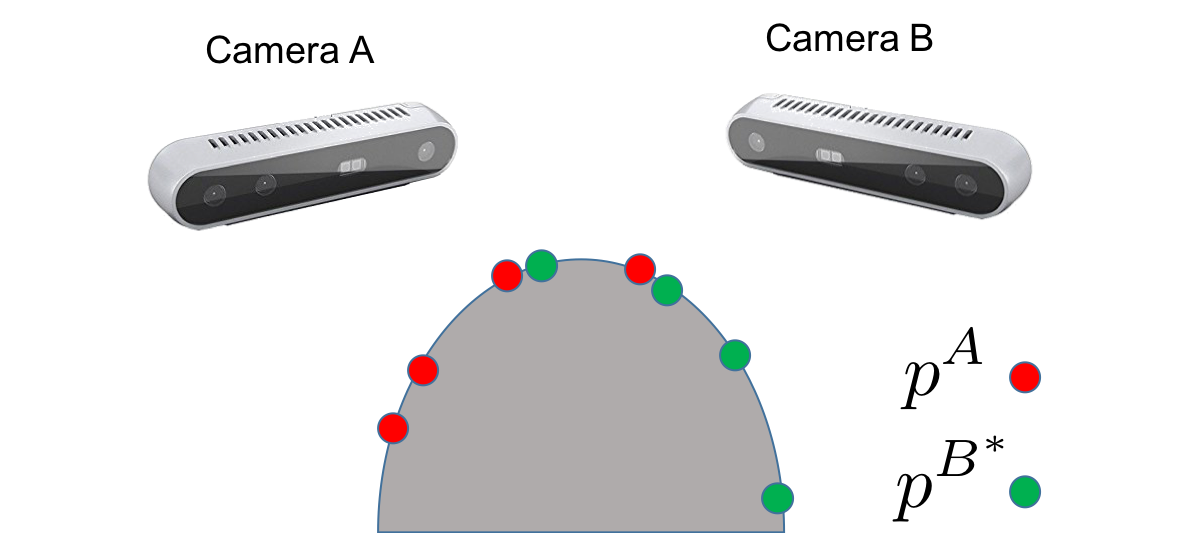
\includegraphics[width=\textwidth]{figures/common2.png}
        \end{subfigure}
        \begin{subfigure}[b]{1.4in}                            
                \centering
                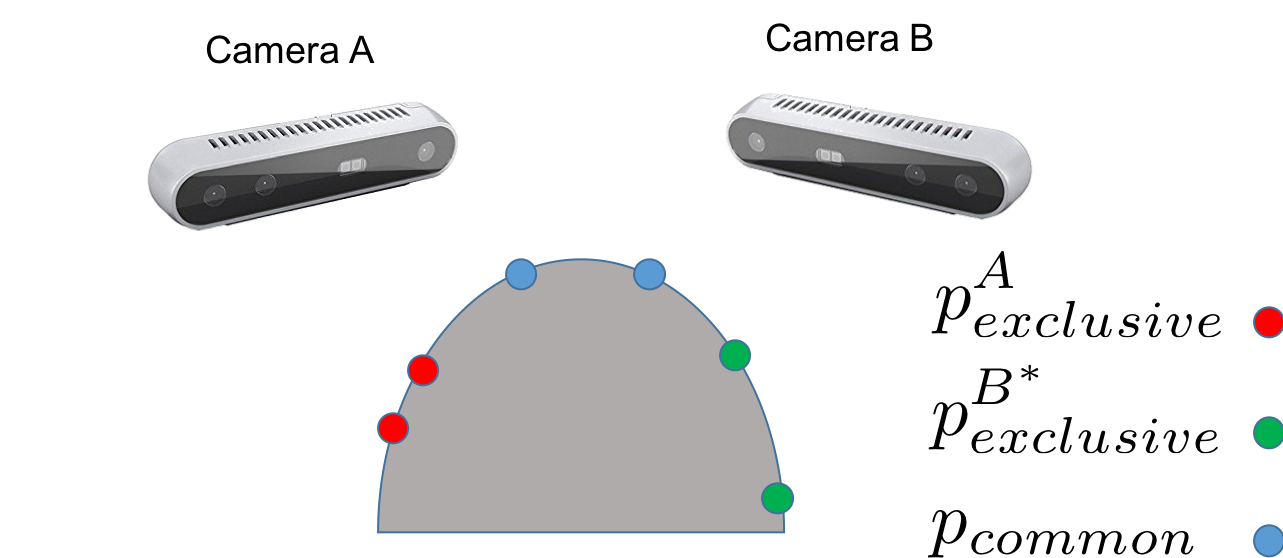
\includegraphics[width=\textwidth]{figures/common1.png}
        \end{subfigure}}}
        \caption{Calibration balls seen from two sensors}
        \label{fig:calib}
\end{figure}

\clearpage
   
\section{Data Driven Inverse Kinematics for Soft Robots}
\blindtext[2]
\subsection{Domain Decomposition of Control Space}
\blindtext[2]
 \begin{figure}[htpb]
        \centering
        \framebox{\parbox{3in}{
        \begin{subfigure}[b]{1.4in} 
                \centering
                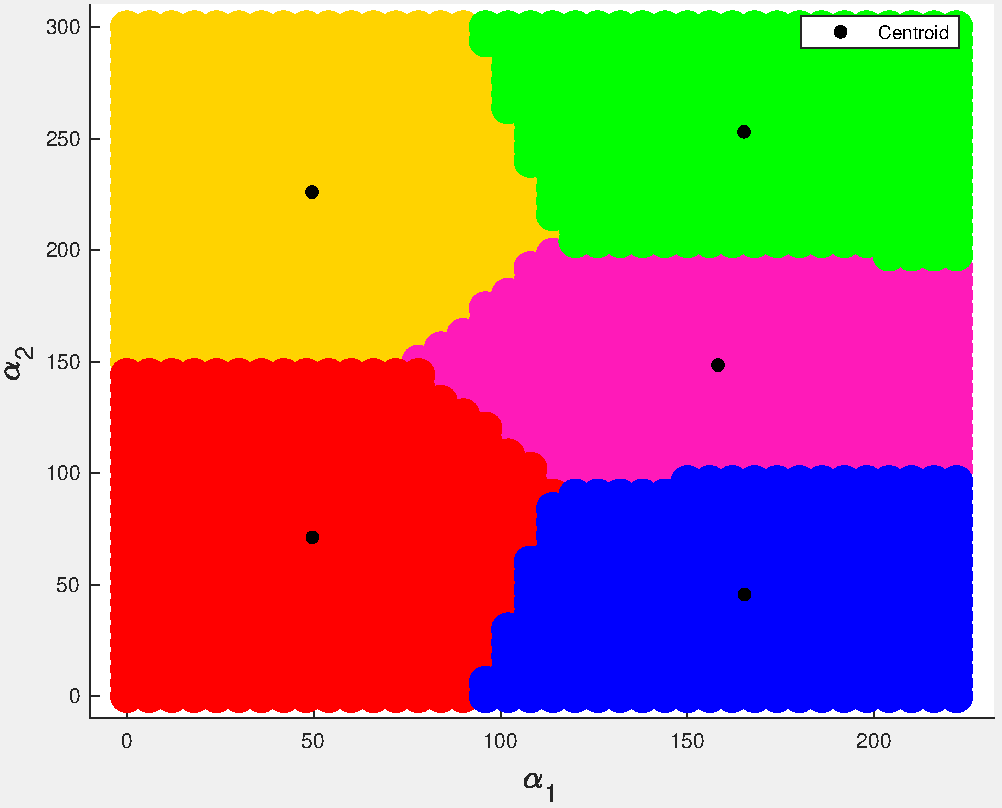
\includegraphics[width=\textwidth]{figures/kmeansseg3.pdf}
        \end{subfigure}
        \begin{subfigure}[b]{1.4in}                            
                \centering
                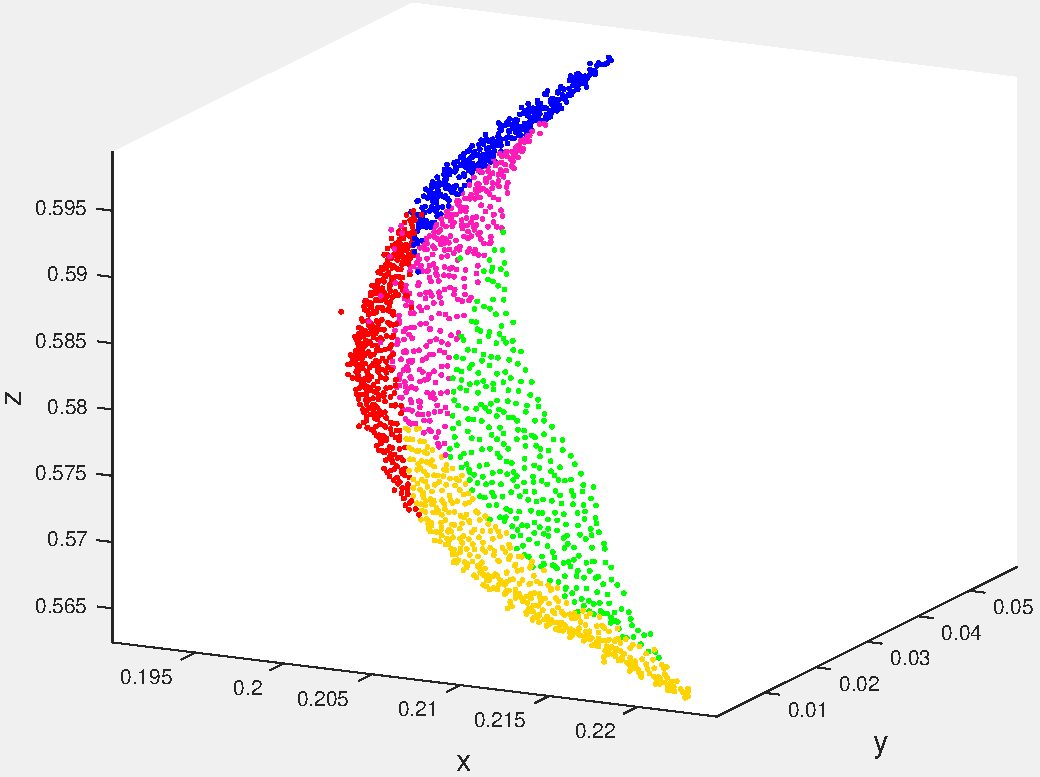
\includegraphics[width=\textwidth]{figures/kmeansseg1.pdf}
        \end{subfigure}}}
        \caption{Calibration balls seen from two sensors}
        \label{fig:calib}
\end{figure}
\blindtext[3]
\subsection{Efficient Polynomial Regression for Higher Order Models}
\blindtext[6]
\begin{figure}[htpb]
      \centering
      \framebox{\parbox{3in}{
        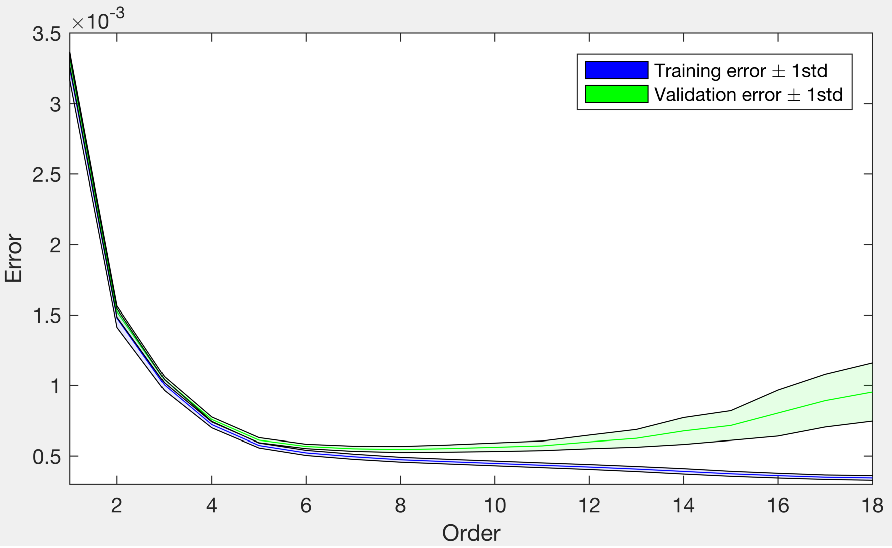
\includegraphics[width=3in]{figures/order_exp.pdf}}}
        \caption{Overview of the LearningCube}
        \label{fig:cube}
\end{figure}
\blindtext[1]
\clearpage

\section{Experiments}

\blindtext[1]
 \begin{figure}[htpb]
        \centering
        \begin{subfigure}[b]{1in} 
                \centering
                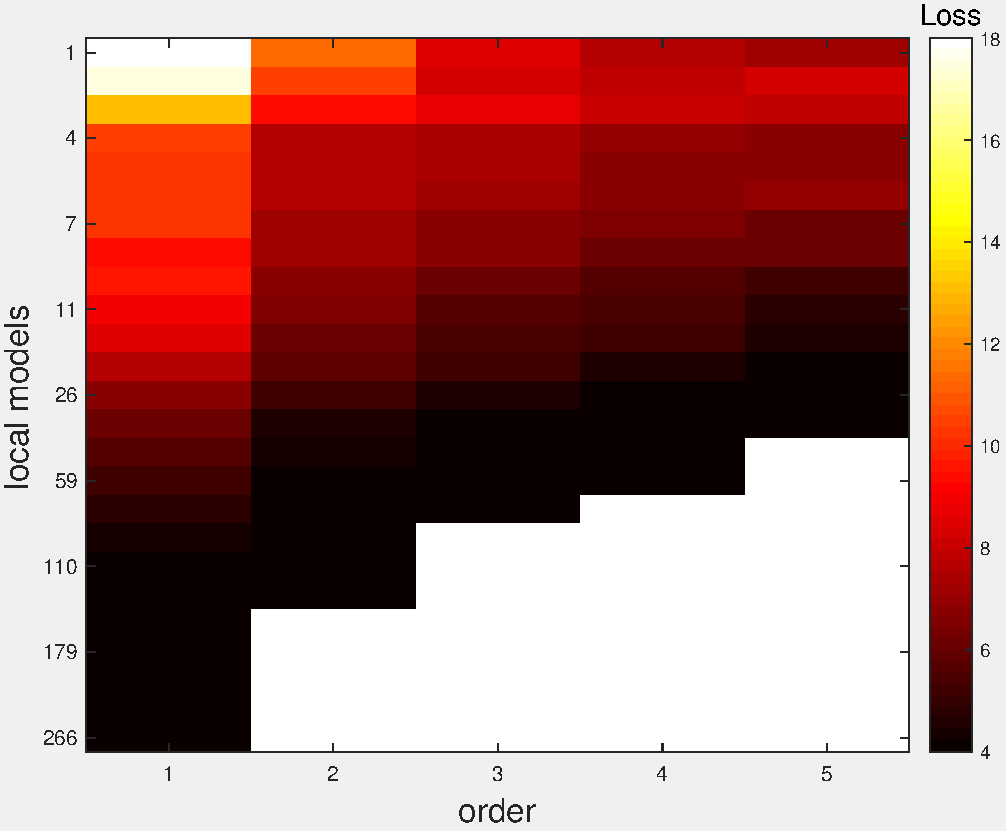
\includegraphics[width=\textwidth]{figures/cross_allQP1.pdf}
                \caption{Training error}
                \label{fig:crossval_train}
        \end{subfigure}
                \begin{subfigure}[b]{1in} 
                \centering
                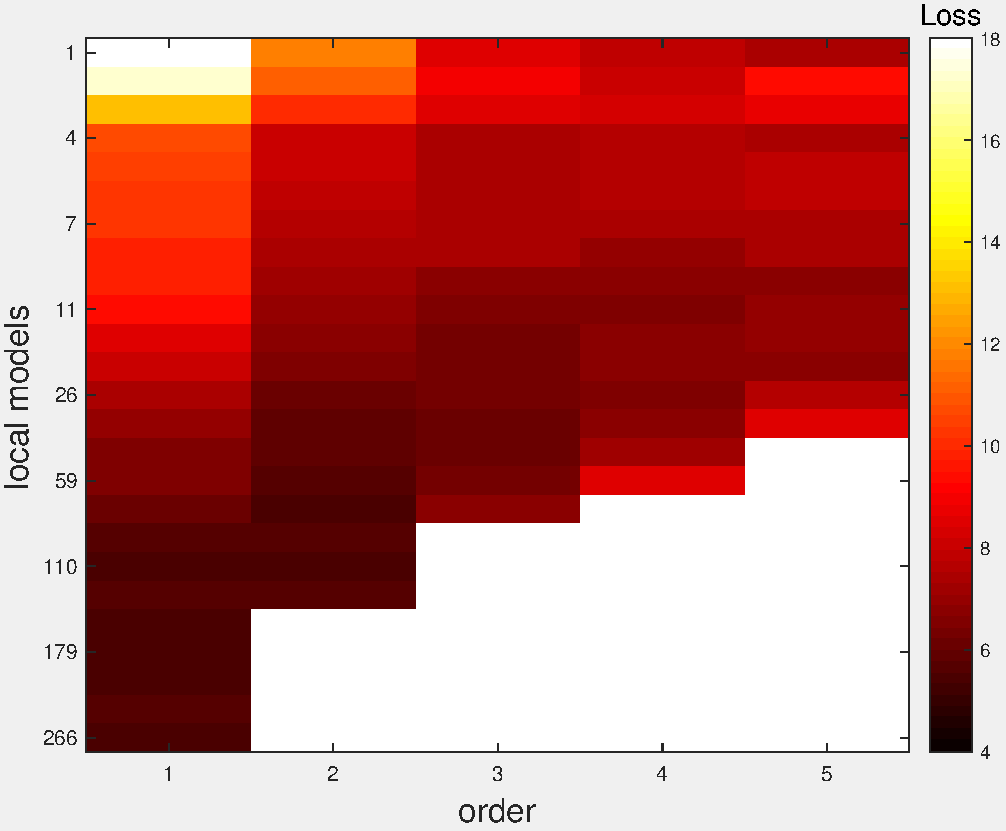
\includegraphics[width=\textwidth]{figures/cross_allQP2.pdf}
                \caption{Validation error}
                \label{fig:crossval_train}
        \end{subfigure}
                \begin{subfigure}[b]{1in} 
                \centering
                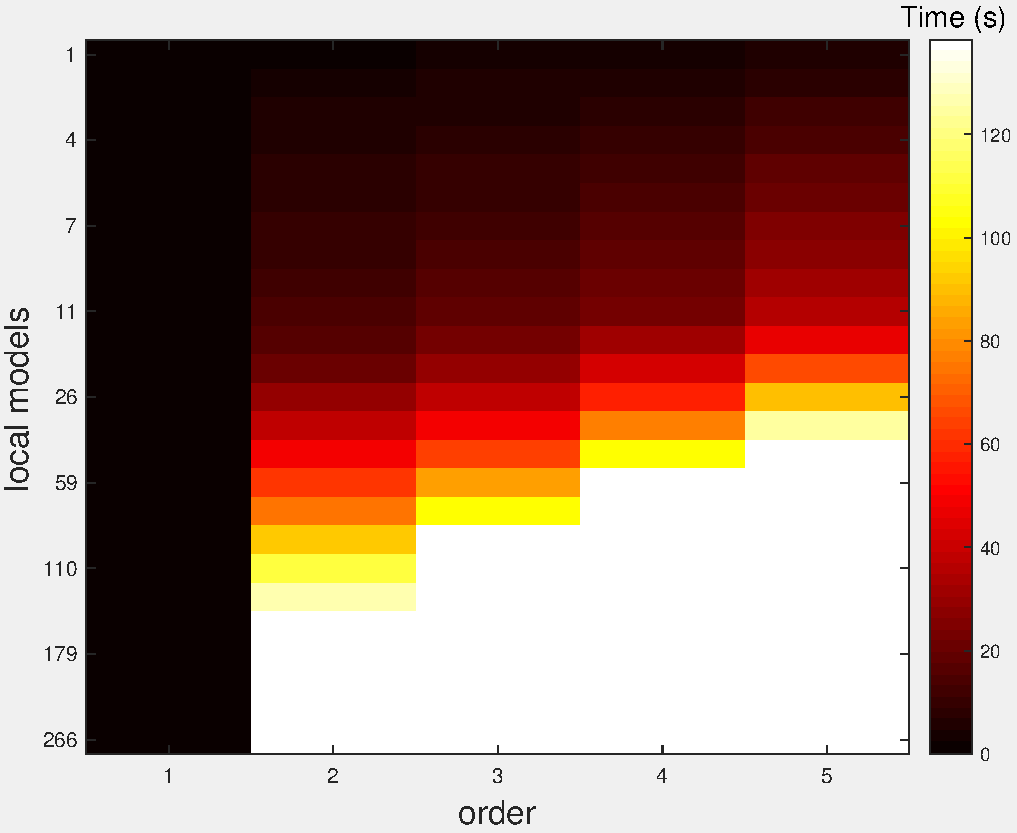
\includegraphics[width=\textwidth]{figures/cross_allQP3.pdf}
                \caption{Execution time}
                \label{fig:crossval_train}
        \end{subfigure}
\end{figure}
\blindtext[1]
 \begin{figure}[htpb]
        \centering
        \begin{subfigure}[b]{1in} 
                \centering
                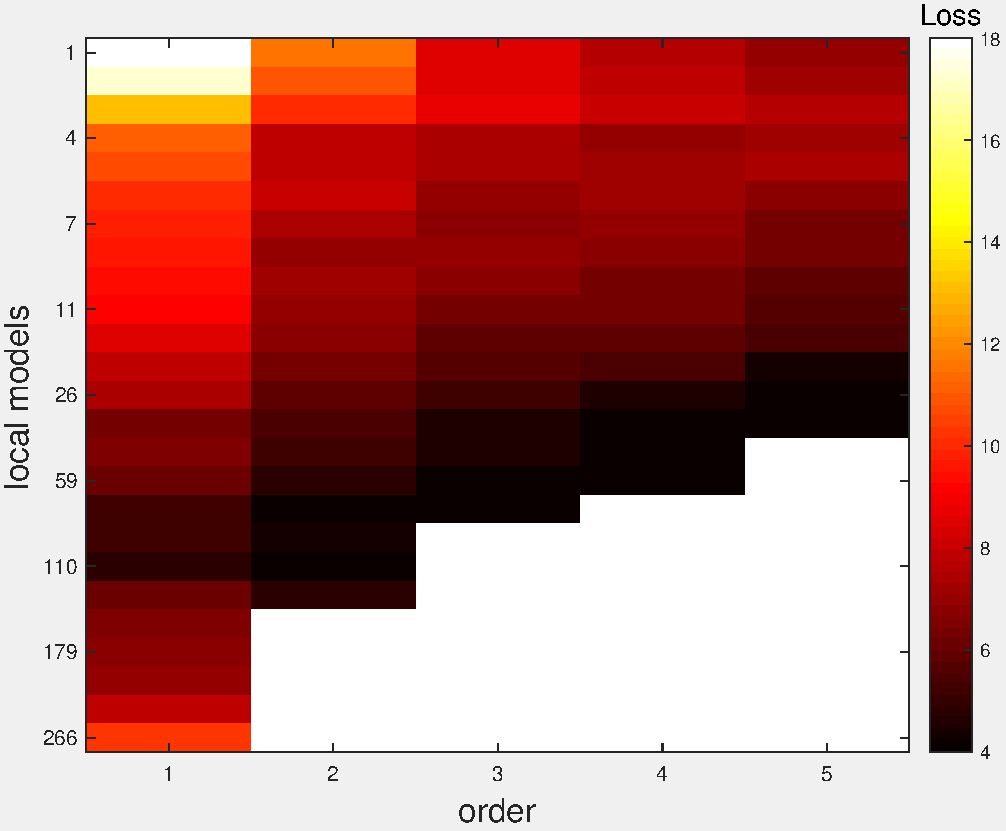
\includegraphics[width=\textwidth]{figures/cross_allreg1.pdf}
                \caption{Training error}
                \label{fig:crossval_train}
        \end{subfigure}
                \begin{subfigure}[b]{1in} 
                \centering
                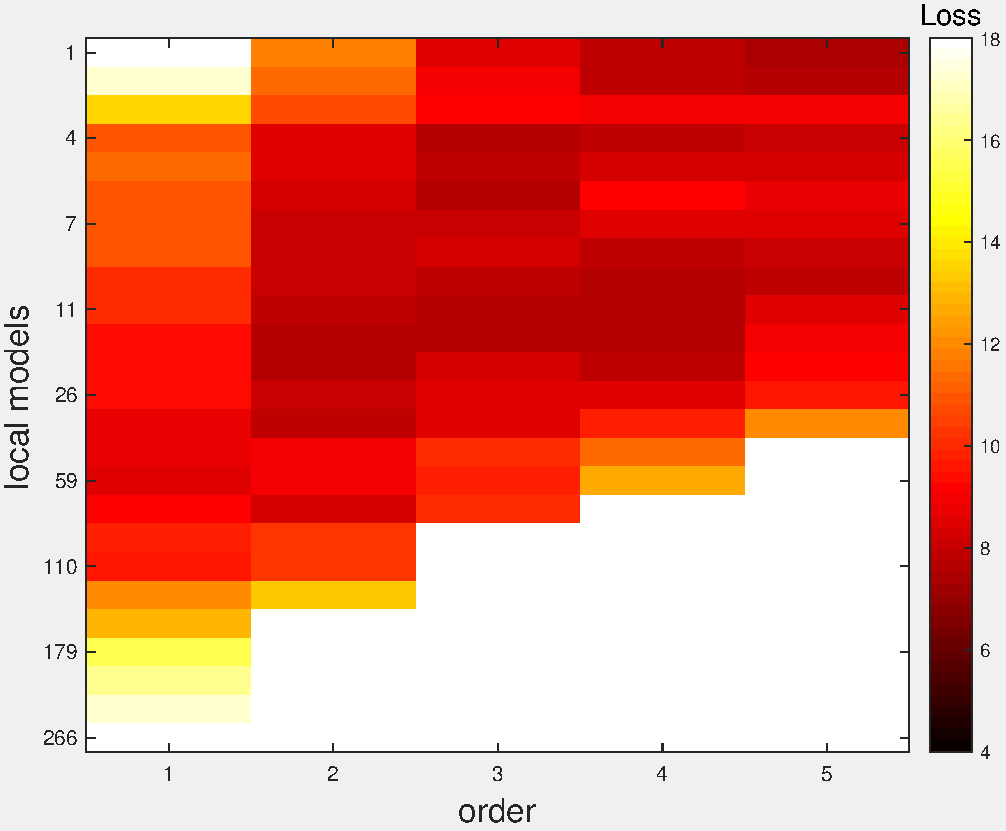
\includegraphics[width=\textwidth]{figures/cross_allreg2.pdf}
                \caption{Validation error}
                \label{fig:crossval_train}
        \end{subfigure}
                \begin{subfigure}[b]{1in} 
                \centering
                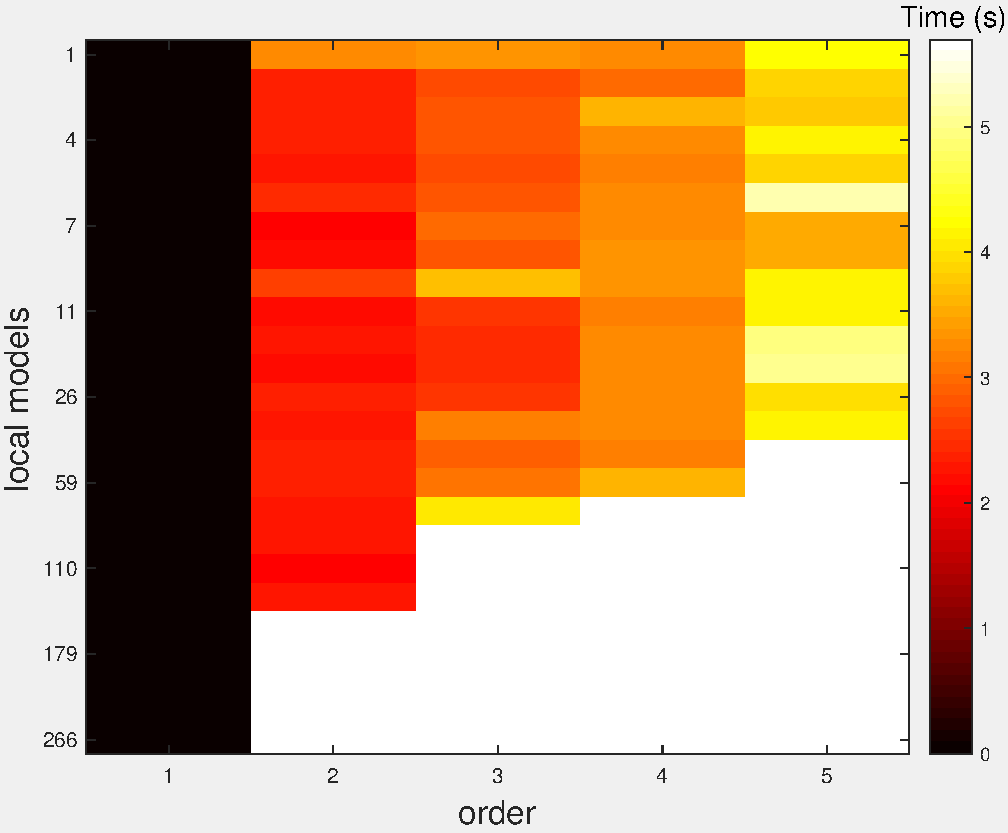
\includegraphics[width=\textwidth]{figures/cross_allreg3.pdf}
                \caption{Execution time}
                \label{fig:crossval_train}
        \end{subfigure}
\end{figure}
\blindtext[1]
 \begin{figure}[htpb]
        \centering
        \begin{subfigure}[b]{0.72in} 
                \centering
                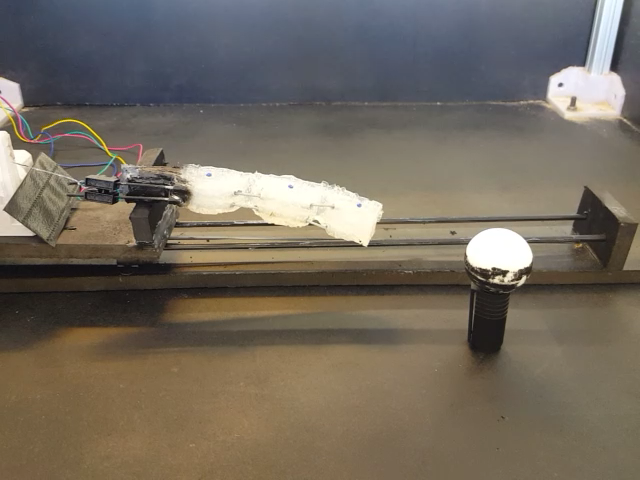
\includegraphics[width=\textwidth]{figures/finger/finger1.png}
        \end{subfigure}
        \begin{subfigure}[b]{0.72in}                            
                \centering
                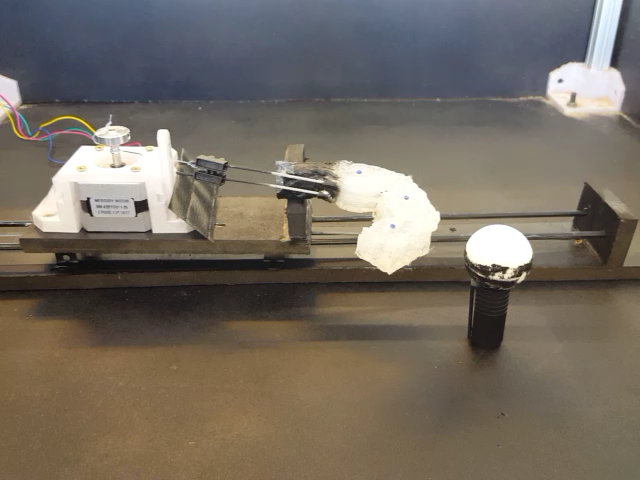
\includegraphics[width=\textwidth]{figures/finger/finger2.png}
        \end{subfigure}
        \begin{subfigure}[b]{0.72in} 
                \centering
                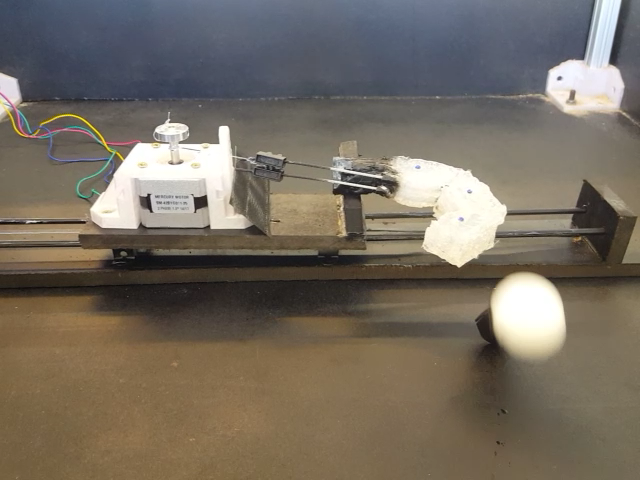
\includegraphics[width=\textwidth]{figures/finger/finger4.png}
        \end{subfigure}
        \begin{subfigure}[b]{0.72in}                            
                \centering
                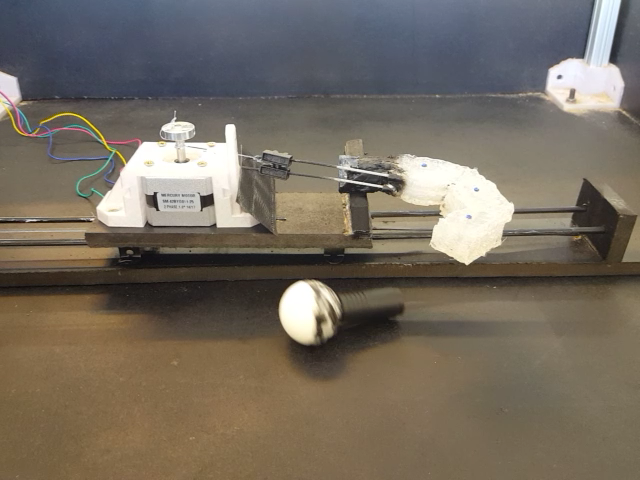
\includegraphics[width=\textwidth]{figures/finger/finger5.png}
        \end{subfigure}
        
        \begin{subfigure}[b]{0.72in} 
                \centering
                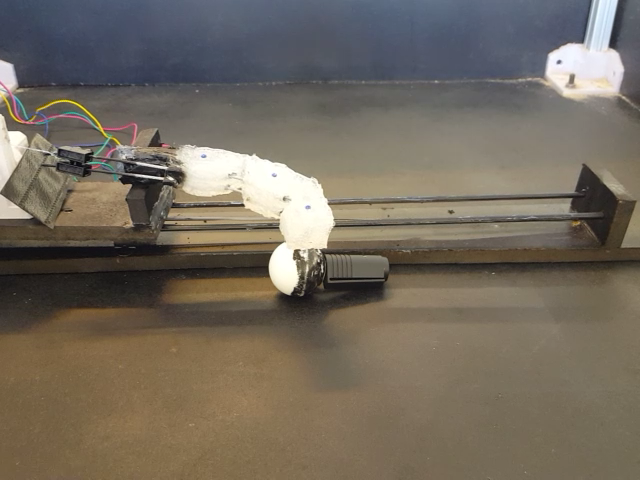
\includegraphics[width=\textwidth]{figures/finger/finger6.png}
        \end{subfigure}
        \begin{subfigure}[b]{0.72in}                            
                \centering
                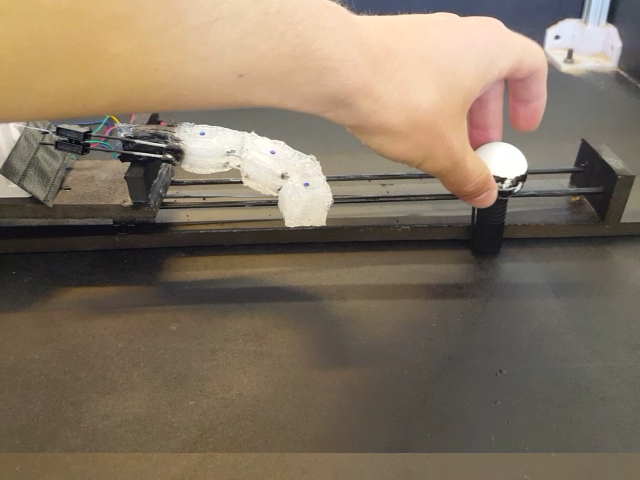
\includegraphics[width=\textwidth]{figures/finger/finger7.png}
        \end{subfigure}
        \begin{subfigure}[b]{0.72in} 
                \centering
                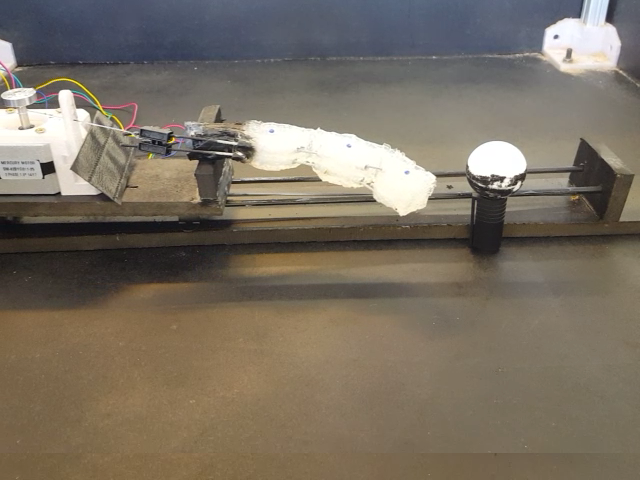
\includegraphics[width=\textwidth]{figures/finger/finger8.png}
        \end{subfigure}
        \begin{subfigure}[b]{0.72in}                            
                \centering
                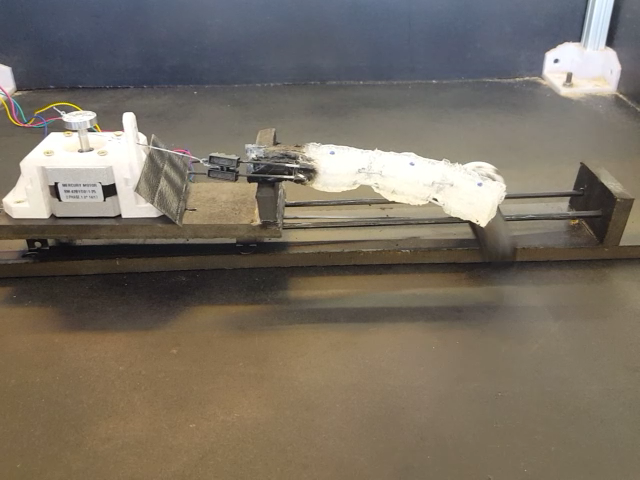
\includegraphics[width=\textwidth]{figures/finger/finger9.png}
        \end{subfigure}
        
        \caption{The finger tries to tip the ball over}
        \label{fig:fingerfun}
        \end{figure}
\blindtext[1]
 \begin{figure}[htpb]
        \centering
        \begin{subfigure}[b]{1.4in} 
                \centering
                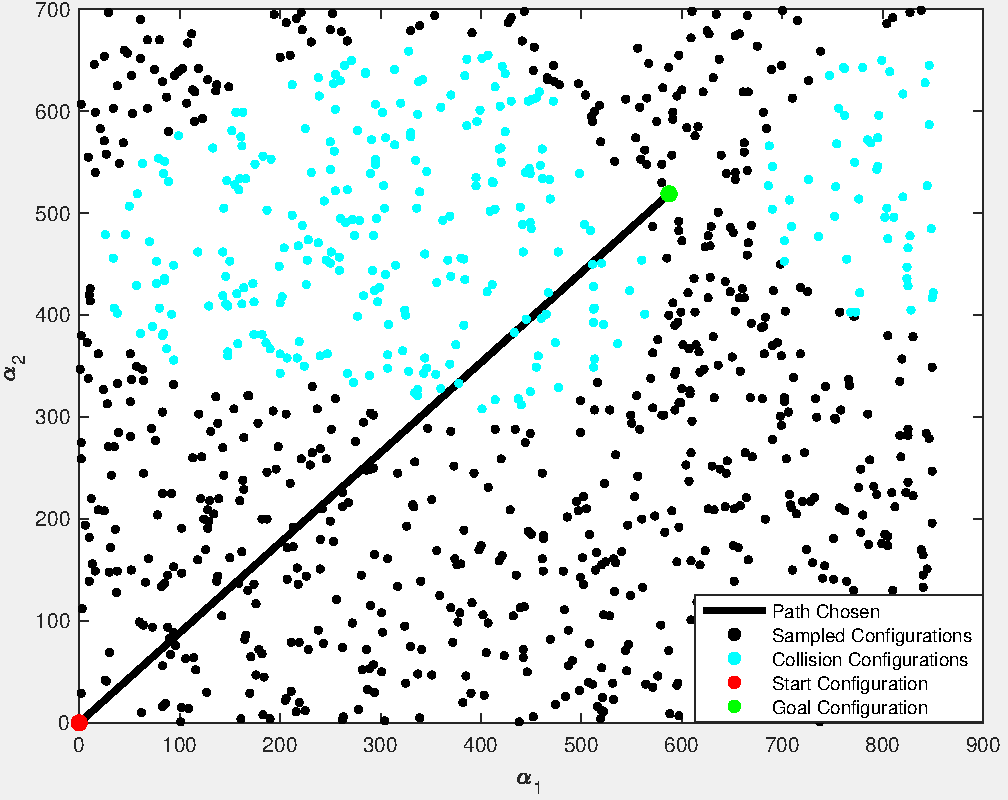
\includegraphics[width=\textwidth]{figures/path/path1.pdf}
                \caption{Naive path}
                \label{fig:path1}
        \end{subfigure}
        \begin{subfigure}[b]{1.4in}                            
                \centering
                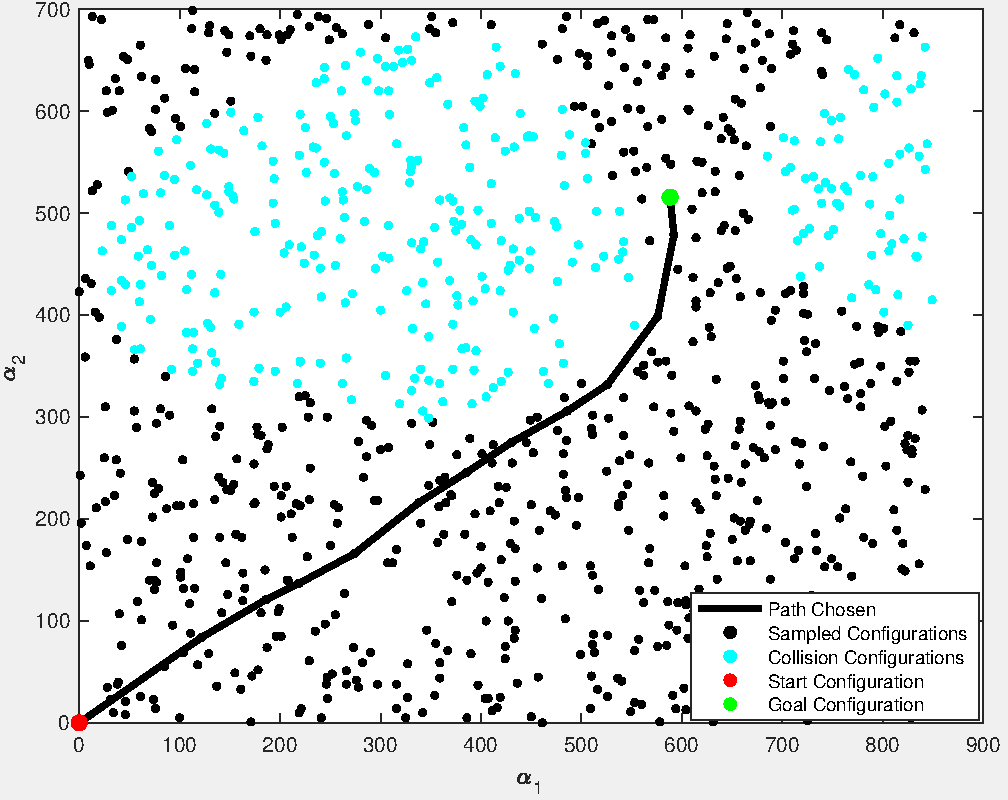
\includegraphics[width=\textwidth]{figures/path/path2.pdf}
                \caption{Collision avoiding path}
                \label{fig:path2}
        \end{subfigure}
        
        \begin{subfigure}[b]{1.4in} 
                \centering
                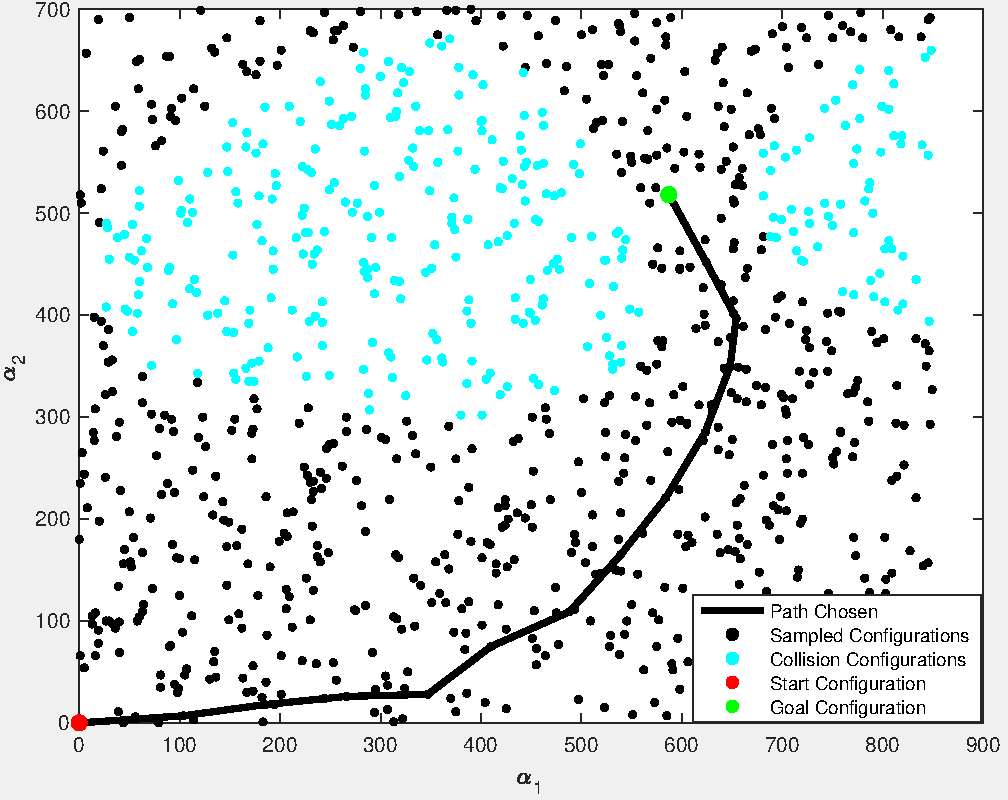
\includegraphics[width=\textwidth]{figures/path/path3.pdf}
                \caption{Minimize probability of collision}
                \label{fig:path3}
        \end{subfigure}
        \begin{subfigure}[b]{1.4in}                            
                \centering
                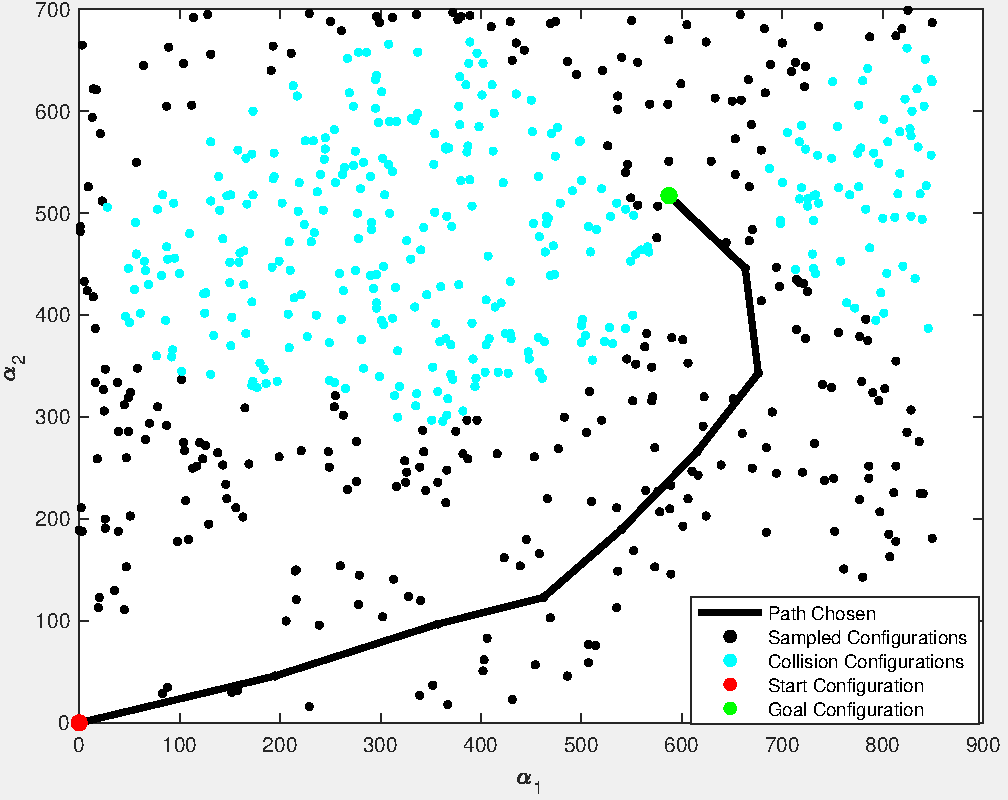
\includegraphics[width=\textwidth]{figures/path/path4.pdf}
                \caption{Importance sampled}
                \label{fig:path4}
        \end{subfigure}
        \caption{Paths through the configuration space}
        \label{fig:path}
\end{figure}

 \begin{figure}[htpb]
        \centering
        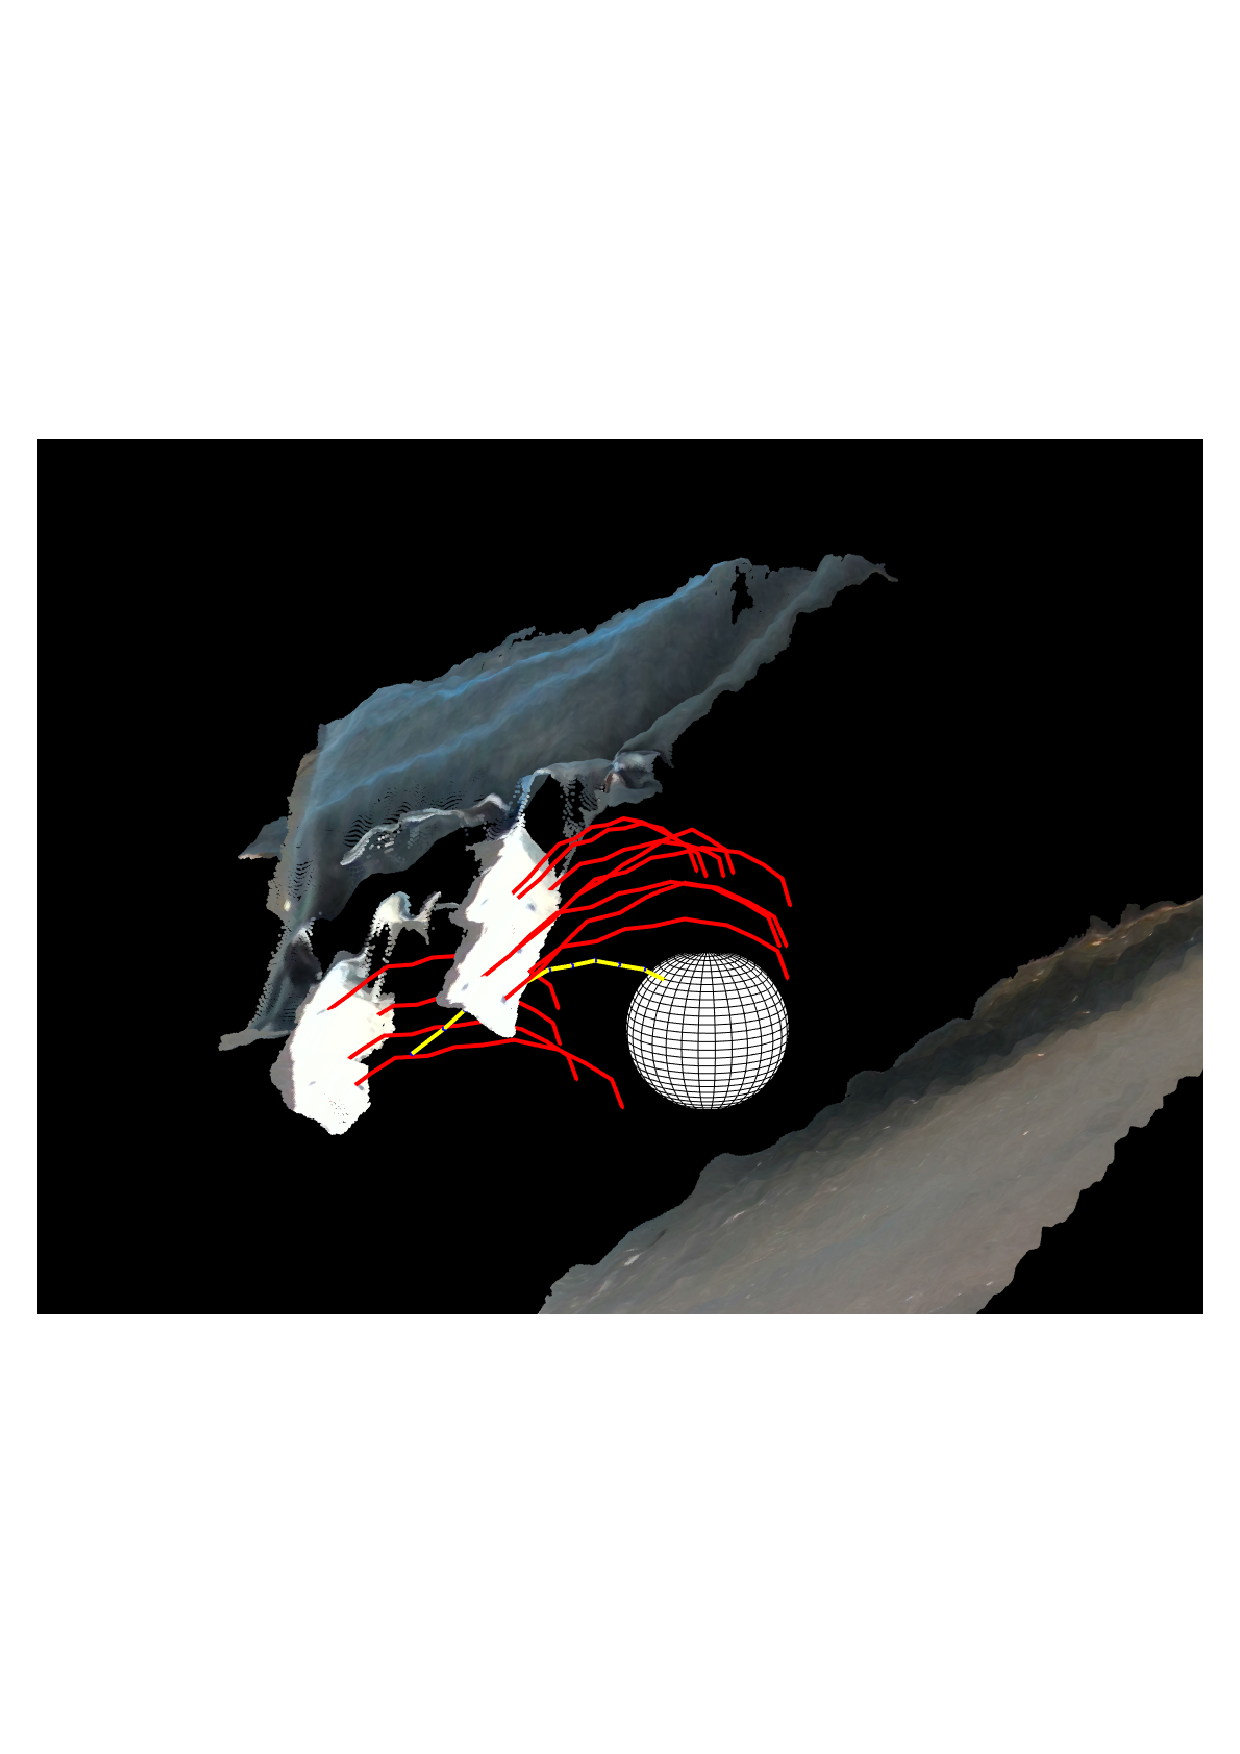
\includegraphics[trim={0 9cm 0 9cm},clip,width=0.5\textwidth]{figures/path/path55.pdf}
        \caption{Trajectory of real markers (red) and phantom marker (yellow) in work-space.}
        \label{fig:work}
\end{figure}

 \begin{figure}[htpb]
        \centering
        \begin{subfigure}[b]{0.72in} 
                \centering
                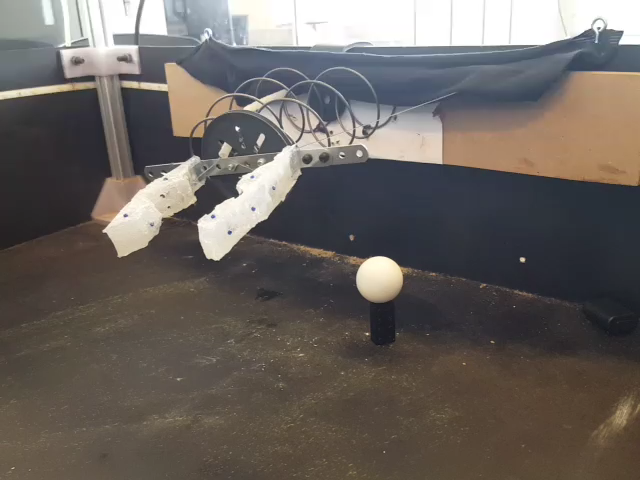
\includegraphics[width=\textwidth]{figures/path/g1.png}
        \end{subfigure}
        \begin{subfigure}[b]{0.72in}                            
                \centering
                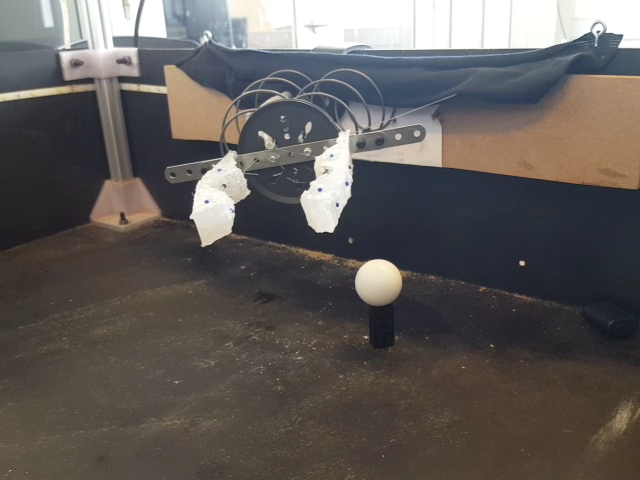
\includegraphics[width=\textwidth]{figures/path/g2.png}
        \end{subfigure}
        \begin{subfigure}[b]{0.72in} 
                \centering
                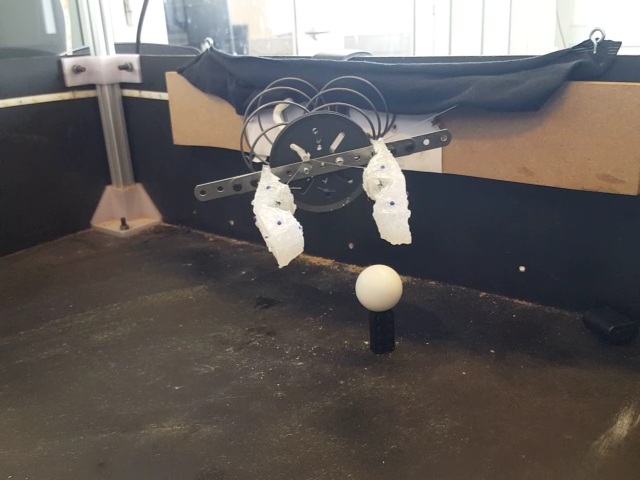
\includegraphics[width=\textwidth]{figures/path/g3.png}
        \end{subfigure}
        \begin{subfigure}[b]{0.72in}                            
                \centering
                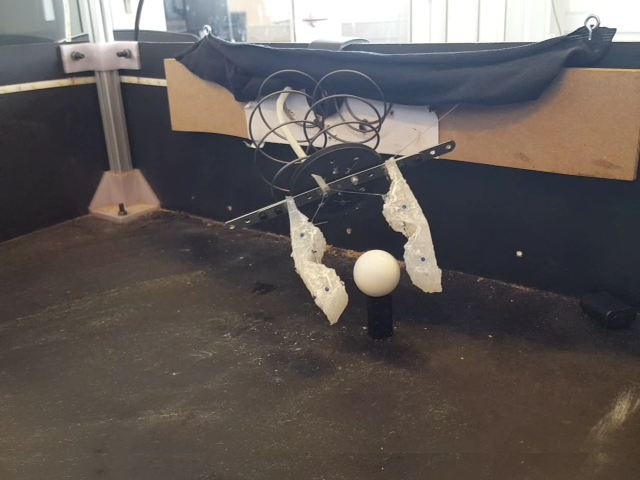
\includegraphics[width=\textwidth]{figures/path/g4.png}
        \end{subfigure}
        \caption{Grabber choosing collision free trajectory}
        \label{fig:grabberpath}
\end{figure}
\blindtext[4]
\section{Discussion and Conclusion}
\blindtext[4]

\addtolength{\textheight}{-12cm}   


\begin{thebibliography}{99}

\bibitem{c1} G. O. Young, ÒSynthetic structure of industrial plastics (Book style with paper title and editor),Ó 	in Plastics, 2nd ed. vol. 3, J. Peters, Ed.  


\end{thebibliography}




\end{document}
